\def\xlist{4}
\def\ylist{4}

\newcommand{\fillrandomly}[4]{
    \pgfmathsetmacro\diameter{#3*2}
    % \draw (0-#3,0-#3) rectangle (#1+#3,#2+#3);
    \foreach \i in {1,...,#4}{
        \pgfmathsetmacro\x{rnd*#1}
        \pgfmathsetmacro\y{rnd*#2}
        \xdef\collision{0}
        \foreach \element [count=\i] in \xlist{
            \pgfmathtruncatemacro\j{\i-1}
            \pgfmathsetmacro\checkdistance{ sqrt( ({\xlist}[\j]-(\x))^2 + ({\ylist}[\j]-(\y))^2 ) }
            \ifdim\checkdistance pt<\diameter pt
                \xdef\collision{1}
                \breakforeach
            \fi
        }
        \ifnum\collision=0
            \xdef\xlist{\xlist,\x}
            \xdef\ylist{\ylist,\y}
            \pgfmathsetmacro\randomvalue{rnd*360}
            \draw [black, line width=2pt, -latex] (\x,\y) +(\randomvalue:-#3) -- +(\randomvalue:#3);
        \fi 

    }
}

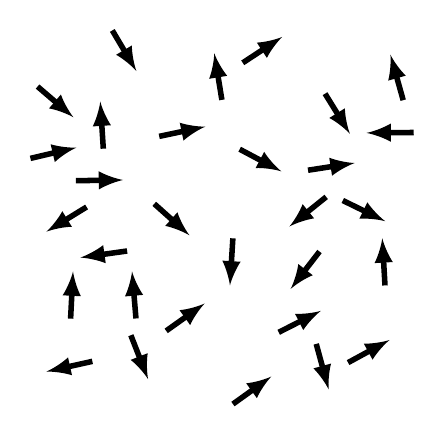
\begin{tikzpicture}[scale=0.6]
\pgfmathsetseed{2}
\fillrandomly{7.5}{7.5}{0.5}{100}
\end{tikzpicture}